\question{13.15}{
    Er is een onderzoek gehouden naar het verband tussen motorinhoud en maximumsnelheid van personenauto's.
    Er werden tien auto's getest.
    De resultaten waren als volgt:
    \begin{center}
        \begin{tabular}{ccc}
            \toprule
                {\bfseries Auto nr.} & {\bfseries Cilinderinhoud} & {\bfseries Max. snelheid (km/uur)} \\            
            \cmidrule{1-1} \cmidrule{2-2} \cmidrule{3-3}
                $I$ & $1,2$ & $140$ \\
                $II$ & $0,8$ & $110$ \\
                $III$ & $0,8$ & $100$ \\
                $IV$ & $2,0$ & $180$ \\
                $V$ & $1,4$ & $150$ \\
                $VI$ & $1,0$ & $100$ \\
                $VII$ & $1,6$ & $160$ \\
                $VIII$ & $1,8$ & $190$ \\
                $IX$ & $1,3$ & $140$ \\
                $X$ & $1,1$ & $130$ \\
            \bottomrule
        \end{tabular}
    \end{center}
}
\begin{enumerate}[label=(\alph*)]
    \item Teken de gegevens in een spreidingsdiagram.
    \answer{
        Bij het tekenen van een spreidingsdiagram is het belangrijk om van te voren te bepalen welke variabele de verklarende (onafhankelijke) variabele  $X$ is en welke variabele de te verklaren (afhankelijke) variabele $Y$ is.
        In dit geval is het het meest logisch om aan de hand van de cilinderinhoud te bepalen wat de te bereiken maximum snelheid is van een auto.
        \begin{center}
            \resizebox{0.9\textwidth}{!}{
                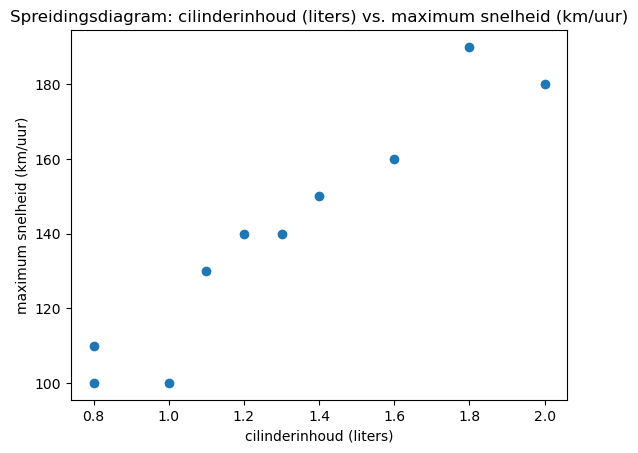
\includegraphics{opg13.15a.png}
            }
        \end{center}
    }

    \item Bepaal het verband tussen de variabelen met behulp van lineaire regressie.
    \answer{
        Uit het spreidingsdiagram is op te merken dat het verband tussen de variabelen cilinderinhoud en maximum snelheid redelijk lineair is.
        Er valt dus zeker iets te zeggen voor de keuze om lineaire regressie toe te passen.

        Om de bijbehorende regressielijn te bepalen, construeren we allereerst de rekentabel met de gemiddeldes $\overline{x}$, $\overline{y}$, $\overline{xy}$, $\overline{x^2}$ en $\overline{y^2}$:

        \begin{center}
            \begin{tabular}{ccccc}
                \toprule
                    $x$ & $y$ & $xy$ & $x^2$ & $y^2$ \\
                \midrule
                    $1,2$ & $140$ & $168$ & $1,44$ & $19600$ \\
                    $0,8$ & $110$ & $88$  & $0,64$ & $12100$ \\
                    $0,8$ & $100$ & $80$  & $0,64$ & $10000$ \\
                    $2,0$ & $180$ & $360$ & $4,0$  & $32400$ \\
                    $1,4$ & $150$ & $210$ & $1,96$ & $22500$ \\
                    $1,0$ & $100$ & $100$ & $1,0$  & $10000$ \\
                    $1,6$ & $160$ & $256$ & $2,56$ & $25600$ \\
                    $1,8$ & $190$ & $342$ & $3,24$ & $36100$ \\
                    $1,3$ & $140$ & $182$ & $1,69$ & $19600$ \\
                    $1,1$ & $130$ & $143$ & $1,21$ & $16900$ \\
                \midrule
                    $\overline{x} = 1,3$ & $\overline{y} = 140$ & $\overline{xy} = 192,9$ & $\overline{x^2} = 1,838$ & $\overline{y^2} = 20480$ \\
                \bottomrule
            \end{tabular}
        \end{center}
        
        Op basis van de bovenstaande tabel kunnen we de co\"effici\"enten $a$ en $b$ van de regressielijn bepalen:
        \begin{align*}
            b   &= \frac{\overline{xy} - \overline{x} \cdot \overline{y}}{\overline{x^2} - (\overline{x})^2} \\
                &= \frac{192,9 - 1,3 \cdot 140}{1,838 - (1,3)^2} \\
                &= \frac{10,9}{0,148} \approx 73,6486 \\
            a   &= \overline{y} - b \cdot \overline{x} \\
                &= 140 - 73,6486 \cdot 1,3 \\
                &\approx 44,2568.
        \end{align*}
        De formule van de regressielijn behorende bij deze steekproef is dus gelijk aan $Y = 44,2568+73,6486X$.

        \begin{center}
            \resizebox{0.9\textwidth}{!}{
                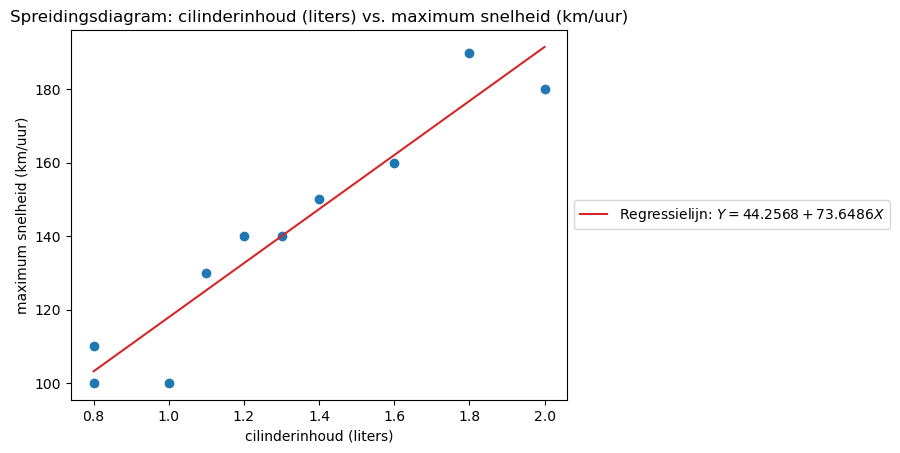
\includegraphics{opg13.15b.png}
            }
        \end{center}
    }

    \item Voorspel aan de hand van en de gevonden lijn de maximumsnelheid van een auto met een cilinderinhoud van $1,5$ liter.
    \answer{
        Aan de hand van de regressielijn kunnen we een voorspelling doen voor de maximumsnelheid van een auto met een cilinderinhoud van $1,5$ liter.
        Dit doen we door simpelweg $X = 1,5$ in te vullen en de bijbehorende $Y$-waarde te berekenen:
        \begin{align*}
            Y = a + b \cdot X = 44,2568 + 73,6486 \cdot 1,5 = 154,7297.
        \end{align*}
        De verwachting is dus dat een willekeurige auto met een cilinderinhoud van $1,5$ liter een maximumsnelheid heeft van $155$ kilometer per uur.
        \begin{center}
            \resizebox{0.9\textwidth}{!}{
                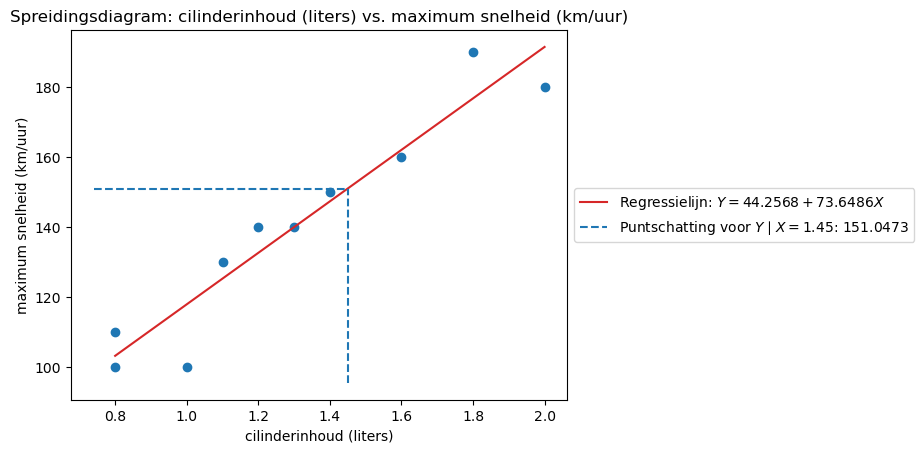
\includegraphics{opg13.15c.png}
            }
        \end{center}
    }

    \item Geef een schatting van de variantie van de storingsterm.
    \answer{
        Bij lineaire regressie nemen we aan dat de storingsterm $\varepsilon$ normaal verdeeld is met verwachtingswaarde $\mu_{\varepsilon} = 0$ en (onbekende) standaardafwijking $\sigma_{\varepsilon}$.
        We kunnen een schatting van de variantie $\sigma^2$ berekenen aan de hand van de volgende formule:
        \begin{align*}
            s_{\varepsilon}^2 &= \frac{n}{n-2} \cdot \left( \overline{y^2} - a \cdot \overline{y} - b \cdot \overline{xy} \right) \\ 
                              &= \frac{10}{8} \cdot \left( 20480 - 44,2568 \cdot 140 - 73,6486 \cdot 192,9 \right) \\ 
                              &\approx 96,5372.
        \end{align*}
    }

    \item Geef een \SI{95}{\percent}-voorspellingsinterval voor de maximumsnelheid van een auto waarvan is gegeven dat deze een cilinderinhoud van $1,45$ liter heeft.
    \answer{
        We willen een voorspellingsinterval bepalen voor de maximumsnelheid van een willekeurige auto met een cilinderinhoud van $1,45$ liter.

        De eerste stap is om de puntschatting voor $Y$ te bepalen aan de hand van de regressielijn $Y = 44,2568+73,6486 \cdot X$ door $X = 1,45$ in te vullen.
        Dit geeft ons een puntschatting van $y_0 = 44,2568 +73,6486 \cdot 1,45 \approx 151,0473$.
        Daarnaast kunnen we de standaardafwijking $\sigma$ van de storingsterm $\varepsilon$ schatten:
        \begin{align*}
            s_{\varepsilon} &= \sqrt{ \frac{n}{n-2} \cdot \left( \overline{y^2} - a \cdot \overline{y} - b \cdot \overline{xy} \right) } \\ 
                            &= \sqrt{ \frac{10}{8} \cdot \left( 20480 - 44,2568 \cdot 140 - 73,6486 \cdot 192,9 \right) } \\ 
                            &\approx 9,8253. 
        \end{align*}

        Vervolgens kunnen we een puntschatting berekenen van de standaardafwijking van $Y$ voor gegeven $X = x_0$:
        \begin{align*}
            s_{f} &= s_{\varepsilon} \cdot \sqrt{ 1 + \frac{1}{n} \cdot \left( 1 + \frac{(x_0 - \overline{x})^2}{\overline{x^2} - \overline{x}^2} \right) } \\
                    &= 9,8253 \cdot \sqrt{ 1 + \frac{1}{10} \cdot \left( 1 + \frac{(1,45 - 1,3)^2}{1,838 - 1,3^2} \right) } \\
                    &\approx 10,3759.         
        \end{align*}

        Omdat we de standaardafwijkingen geschat hebben en de storingstermen normaal verdeeld zijn, moeten we werken met de $t$-verdeling met $df = n - 2 = 8$ vrijheidsgraden.
        De $t$-waarde die hoort bij een betrouwbaarheidsniveau $\alpha = 0,05$ is gelijk aan
        \[
            t = \invt(\text{opp} = 1 - \alpha / 2; \text{df} = n - 2) = \invt(\text{opp} = 0,975; \text{df} = 8) \approx 2,3060.
        \]
        Het \SI{95}{\percent}-betrouwbaarheidsinterval voor de gemiddelde $Y$ voor gegeven $X = 1,45$ kan dus worden beschreven door
        \begin{align*}
                    & [y_0 - t \cdot s_{f}; y_0 - t \cdot s_{f}] \\ 
            &= [151,0473 - 2,3060 \cdot 10,3759; 151,0473 + 2,3060 \cdot 10,3759] \\ 
            &\approx [127,1205; 174,9741]. 
        \end{align*}
        
        Met \SI{95}{\percent} betrouwbaarheid ligt de maximumsnelheid van een willekeurige auto met een cilinderinhoud van $1,45$ liter tussen ongeveer $127$ en $175$ kilometer per uur.
        \begin{center}
            \resizebox{0.9\textwidth}{!}{
                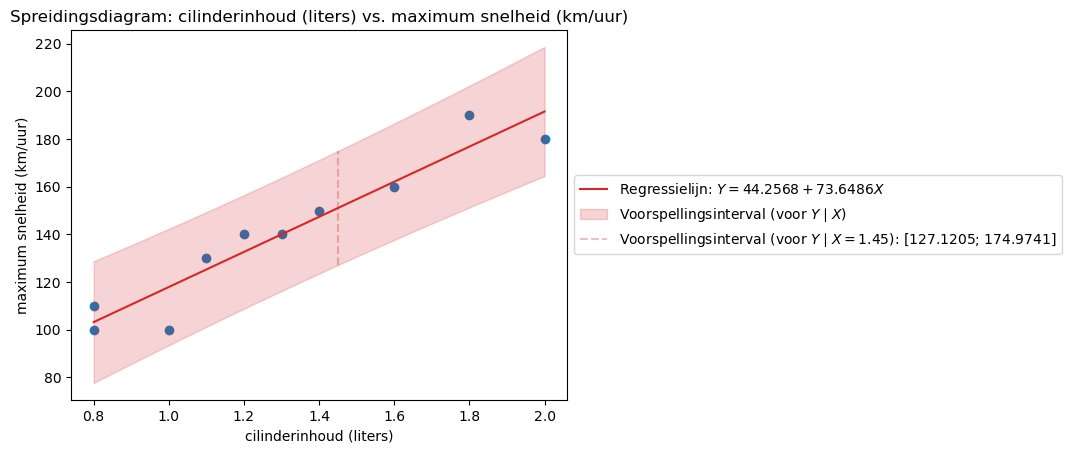
\includegraphics{opg13.15e.png}
            }
        \end{center}
    }
\end{enumerate}